\chapter{Projekt i implementacja}

\section{Wykorzystane technologie}
\subsection{Python 3.8.1}
Do implementacji algorytmu został użyty Python. Jest to najpopularniejszy język programowania w domenie uczenia maszynowego. Wymagana jest wersja 3.8+ ze względu na użycie w implementacji metod dostępnych od tej wersji.  
\subsection{PonyGE2}
PonyGE2 \cite{Fenton_2017} jest implementacja ewolucji genetycznej w jezyku Python. Pozwala na latwa konfiguracje parametrow ewolucji genetycznej oraz latwa mozliwosc dodania wlasnych problemow oraz sposobow ewaluacji wynikow.

\begin{figure}[h]
	\centering{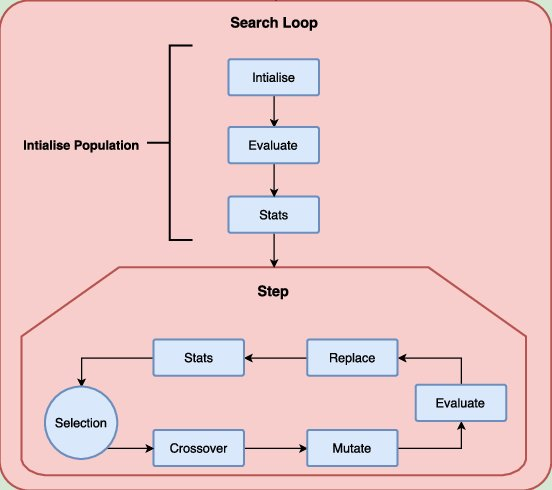
\includegraphics{PonyGE2-search-loop.jpg}}
	\caption{\label{fig:subcaption_example}Pętla wyszukiwania}
\end{figure}

\section{Tworzenie gramatyki procesu biznesowego}

Przy tworzeniu gramatyki procesu biznesowego ważnym jest, żeby znaleźć balans, jeśli chodzi o poziom skomplikowania zaproponowanej
gramatyki.  W pracy \cite{10.1007/978-3-540-69534-9_35} autorzy przeanalizowali składniki języka BPMN pod kątem częstotliwości ich stosowania. z pracy wynika, że najczęściej stosowany elementami modelów procesu biznesowego, jeśli chodzi o bramki są: xor, and oraz pętle lop. Do przedstawionej poniżej gramatyki dodano także bramkę opt, czyli or jako uogólnienie bramki xor w celu uniknięcia zagnieżdżonych bramek xor. Ponadto koniecznym jest posiadanie bramki seq, która oznacza normalny przepływ procesów.

Zapis GE{\_}RANGE:n jest rozszerzenie do gramatyki zapewnianym przez PonyGE2, ktore umożliwia dodanie ilosci zmiennych, czyli GE{\_}RANGE:2 oznacza 0|1|2.
Wzorując się na  Zapis GE{\_}RANGE:dataset{\_}vars jest rozszerzenie do gramatyki zapewnianym przez PonyGE2, ktore umożliwia dodanie ilosci zmiennych odpowiadajacej ich ilosci w zbiorze danych.

\begin{figure}[!ht]
\lstset{caption=Gramatyka procesu biznesowego, captionpos=b}
\lstset{label=src:grammar, frame=single}
\begin{lstlisting}
<e> ::= <slot><slot><anygate><slot><slot>

<anygate> ::=  <anygate><anygate> | <name>(<slots>) | {<event>}

<slot> ::= <anygate> | '' | '' | '' | '' | '' | '' | '' | '' | ''

<slots> ::= <slot><slot><anygate><slot><slot>

<name> ::= and | xor | seq | opt | lo<0_n>

<event> ::= GE_RANGE:dataset_vars

<0_n> ::= GE_RANGE:5
\end{lstlisting}
\end{figure}

Przykład wygenerowanej gramatyki:
and(\{d\}opt(\{f\})and(\{a\}\{c\})lop(seq(lop(\{a\})\{e\})))

Wszystkie bramki mają nazwy tej samej długości - 3 znaki, co pozwoli na łatwiejsze parsowanie gramatyki.

longate - oznacza pętle 
Poniższy przykład pokazuje gramatykę, którą ciężko opisać przy pomocy podstawowych bramek logicznych: 
\begin{figure}[h]
	\centering{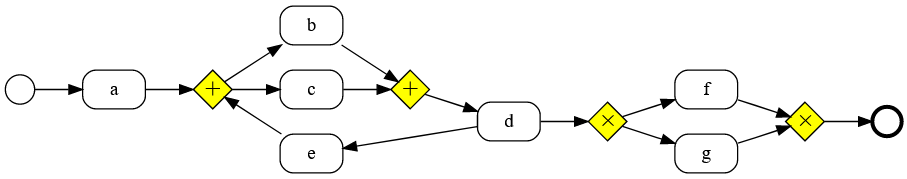
\includegraphics{Grammar-lop-example.png}}
	\caption{\label{fig:subcaption_example}Przykład problemu}
\end{figure}

Jest to możliwe za pomocą notacji: 
\{a\}and(xor(\{b\}\{c\})\{d\})\{e\}lop(\{f\}and(xor(\{b\}\{c\})\{d\})\{e\})xor(\{g\}\{h\})

Użycie powyższej notacji rodzi jednak kilka problemów, Musimy mieć produkcje 
\{a\}lo1(\{f\}and(xor(\{b\}\{c\})\{d\})\{e\})xor(\{g\}\{h\})
\clearpage

\section{Projekt systemu}

\subsubsection{Podział na moduły}

Implementację podzielone na następujące moduły:
\begin{itemize}
    \item wrappers - PonyGE2 nie jest przystosowane do zaimportowania jako biblioteka, dlatego żeby oddzielić kod PonyGE2 od naszego kodu należało rozszerzyć lub nadpisać cześć z modułów PonyGE2. Moduły, które nadpisano to params, który zawiera konfigurację aplikacji oraz grammar, gdzie dodano zmiany w jaki sposób parsowana jest podana gramatyka. 
  \item fitness{\_}functions - zawiera klasę bazowy moduł, gdzie znajduje się bazowa klasa dla obliczania metryk
  \item process{\_}discovery - moduł zawiera całą logikę obliczenia metryk
\end{itemize}


\begin{figure}[!ht]
	\centering{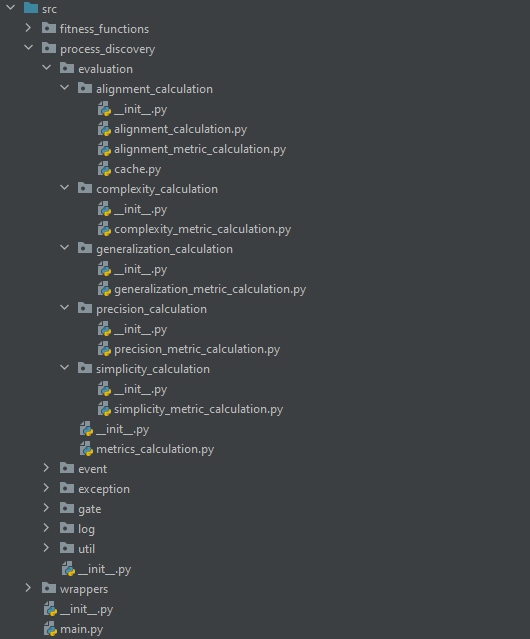
\includegraphics{Modules.png}}
	\caption{\label{fig:flow_chart}Podział na moduły}
\end{figure}

\subsubsection{Model}

Podział na dwie klasy przydatne na różnym etapie procesowania:

Gate:

\begin{figure}[h]
	\centering{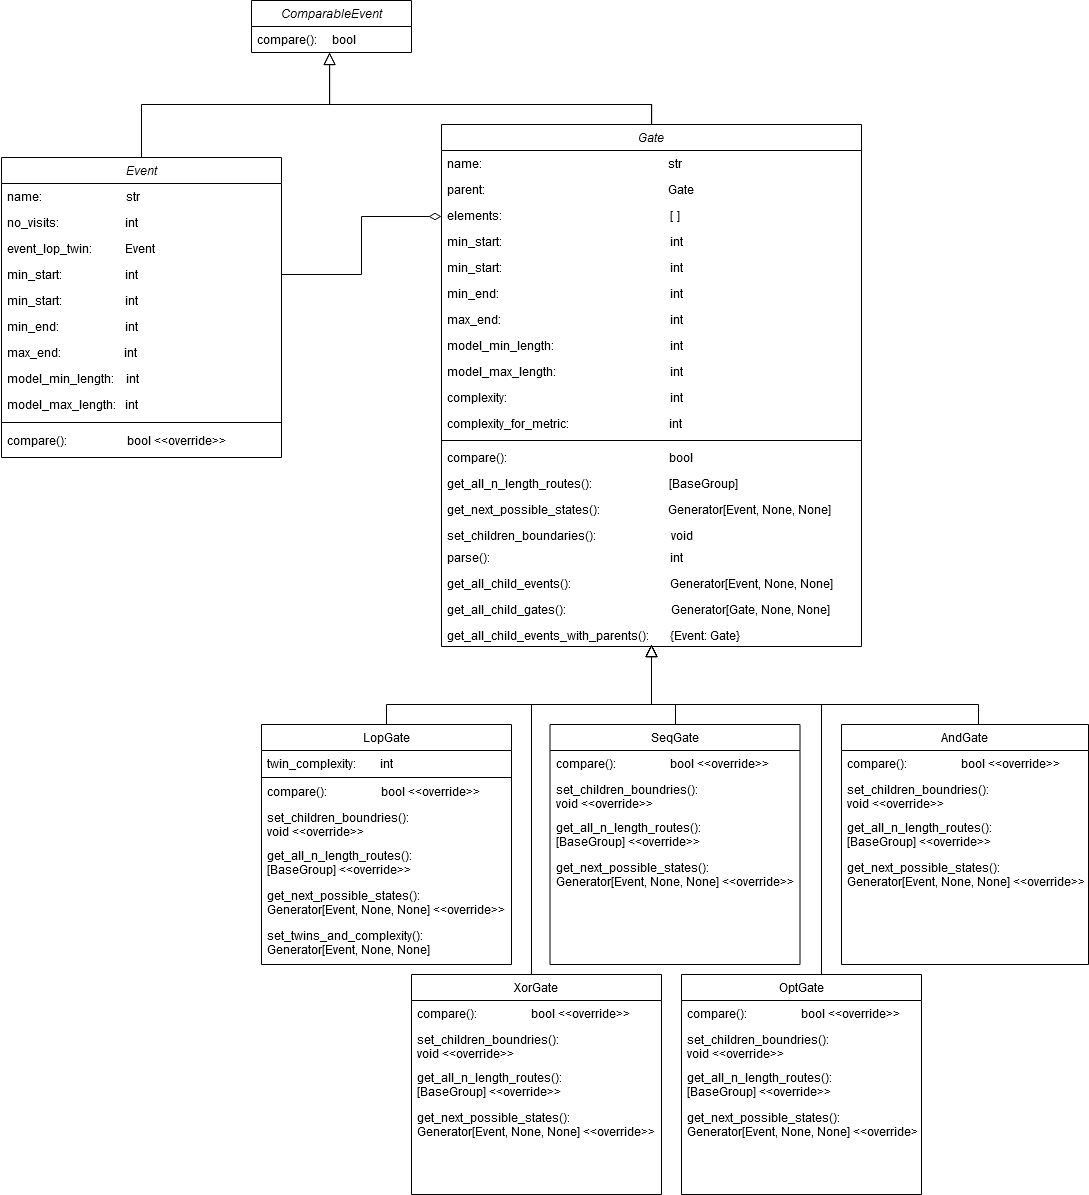
\includegraphics[scale=0.5]{GateUML.png}}
	\caption{\label{fig:subcaption_example}Gate UML}
\end{figure}

Event group:

\begin{figure}[h]
	\centering{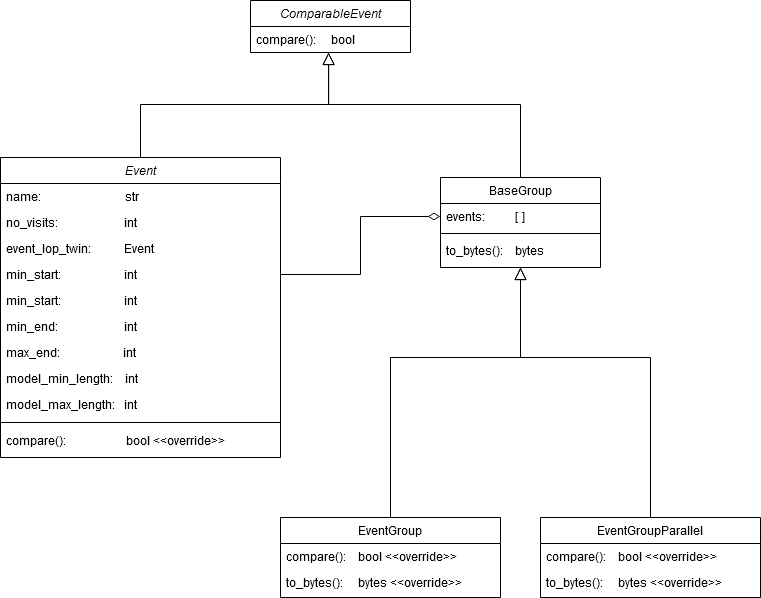
\includegraphics[scale=0.5]{EventUML.png}}
	\caption{\label{fig:subcaption_example}Event UML}
\end{figure}


\section{Implementacja}

\subsubsection{Ogólny schemat blokowy}
\clearpage

\begin{figure}[!ht]
	\centering{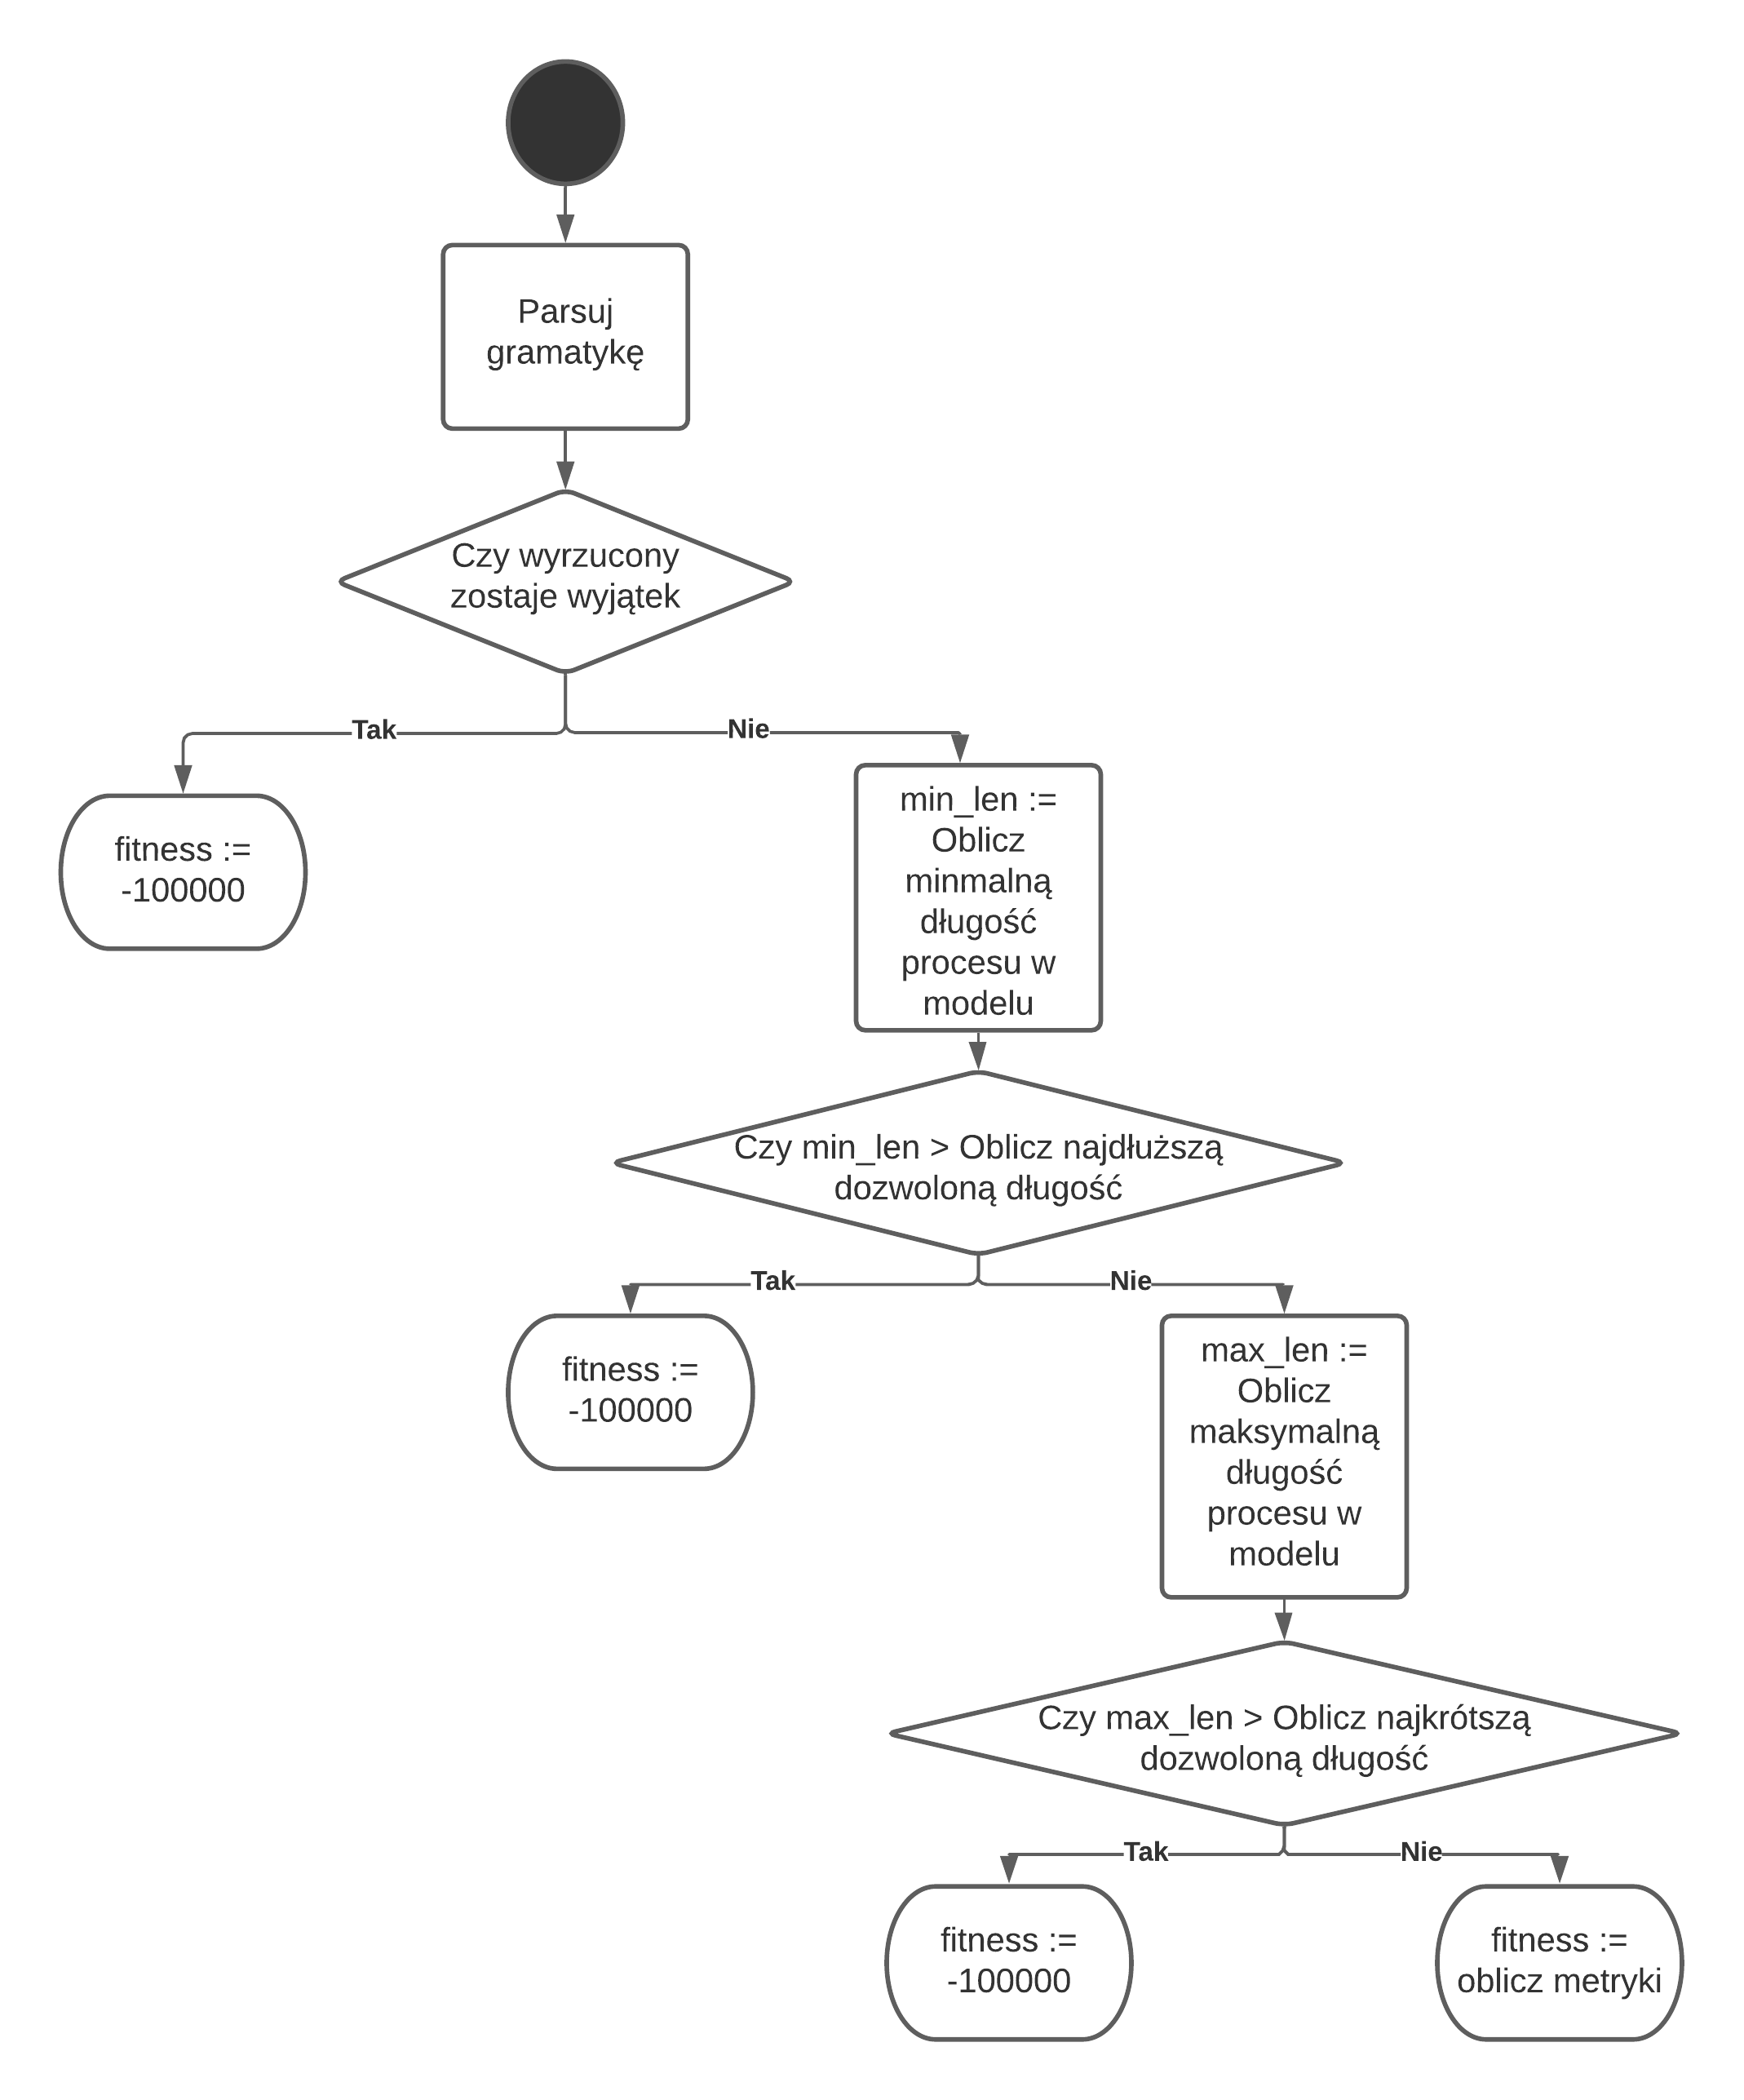
\includegraphics{Overall-flow-chart.png}}
	\caption{\label{fig:flow_chart}Ogólny schemat blokowy}
\end{figure}

\subsubsection{Parsowanie gramatyki}
Parser pozwala na przetworzenie wyników uzyskanych na drodze ewolucji gramatycznej na postać, na której łatwiej będzie operować. Rezultaty uzyskane na drodze rewolucji gramatycznej w PonyGE2 są w formie tekstowej, z którą praca byłaby niewygodna, dlatego używamy parsera, żeby otrzymać wynik w postaci drzewa obiektów Gate, którego liśćmi będą obiekty Event.
Parsując korzystamy z faktu, że przy projektowaniu gramatyki wszystkie bramki logiczne zostały oznaczone 3 literowymi symbolami, a wszystkie zdarzenia otoczone nawiasami klamrowymi. Tworząc każdy obiekt Event dodajemy informację o liczbie dzieci tego obiektu, co przyda nam się przy obliczaniu metryki precyzja.

\begin{figure}[!ht]
\lstset{caption=Parser gramatyki, captionpos=b}
\lstset{label=src:passive, frame=single}
\begin{lstlisting}
    def parsuj(wyrażenie: str) -> int:

        for i w zakresie długość_wyrażenia:
            if wyrażenie[i] == "{":
                zdarzenie := Event(wyrażenia[i + 1])
                dodaj zdarzenie do aktualnie parsowanej bramki 
                i += 2
            elif wyrażenie[i] == ")":
                return i+1
            elif i+4 < długość_wyrażenia:
                if wyrażenie[i:i + 3] == "seq" and (self.name == "seq" or self.name == "lop"):
                    usuń_niepotrzebe_bramki
                else:
                    if wyrażenie[i:i+2] == 'lo' and wyrażenie[i:i+3] != 'lop':
                    
                	    bramka := stwórz nową bramkę Gate typu zgodnego z wyrażeniem 
                	    i += 3
                	    przeparsowane_znaki = bramka.parsuj(wyrażenie[i+4:])
                	    dodaj zdarzenie do aktualnie parsowanej bramki 
                	    i += ilość_przeparsowanych_znaków
            else:
                wyrzuć wyjątek
\end{lstlisting}
\end{figure}

\subsubsection{Obliczanie metryk}
Mając już sparsowany model musimy obliczyć metryki. Najbardziej problematyczną metryką do obliczenia jest dopasowanie. Obliczanie dopasowanie można opisać następującymi krokami:
\begin{itemize}
  \item[•] Znalezienie ścieżek o długości n w modelu.
  \item[•] Przerobienie ścieżek na postać zawierającą BaseGroup.
  \item[•] Obliczenie dopasowania.
\end{itemize}
Metryką, która wymaga 
W pierwszej kolejności obliczamy metrykę dla dopasowania. Wszystkie inne metryki są obliczane dla najlepiej dopasowanej gramatyki.
 
\clearpage
\begin{figure}[!ht]
\lstset{caption=Obliczanie metryk, captionpos=b}
\lstset{label=src:best_result, frame=single}
\begin{lstlisting}
def oblicz_metryki(log_info, model, najkrótsza_dozwolona_długość, 
                   najdłuższa_dozwolona_długość, cache) -> int:
                   
    metryki['PROSTOTA'] = oblicz_metrykę_prostota(lista_zdarzeń_w_procesie), unikalne_zdarzenia_w_logu)
    if metryki['PROSTOTA' < 2/3:
        return 0

    stosunek_wspólnych_zdarzeń_w_logu_i_modelu := 
        oblicz_stosunek_wspólnych_zdarzeń_w_logu_i_modelu()		   
        if stosunek_wspólnych_zdarzeń_w_logu_i_modelu <
            MINIMALNY_STOSUNUK_WSPÓLNYCH_ZDARZEŃ_W_LOGU_I_MODELU:
        return stosunek_wspólnych_zdarzeń_w_logu_i_modelu/10
        
    idealnie_dopasowane_logi := pusty_słownik
    skumulowany_błąd := 0
    
    for proces w log:
        najlepszy_błąd_lokalny, najlepiej_dopasowana_ścieżka, najlepszy_process := 
      	oblicz_metryki_dla_jednego_procesu(proces, model, minimalna_długość, 
      	maksymalna_długość, cache)
    	if jakikolwiek proces w najlepiej_dopasowanej_ścieżce nie znajduje się w modelu:
            value, best_aligned_process = obilcz_dopasowanie_bez_cache(best_event_group, 
                list(process), dict())
            best_local_error = calculate_alignment_metric(value, len(process),
             len(best_event_group))
        if najlepszy_błąd_lokalny == 0:
            idealnie_dopasowane_logi.dodaj()[tuple(best_aligned_process)] = 
            log_info.log[process]
        add_executions(model_events_list, best_aligned_process, log_info.log[process])

	metryki := oblicz_metryki 
	najlepszy_wynik := oblicz_średnią_ważoną_metryk
    return najlepszy_wynik
\end{lstlisting}
\end{figure}

\subsubsection{Obliczanie metryk dla jednego procesu}
\clearpage
\begin{figure}[!ht]
\lstset{caption=Obliczanie metryk dla jednego procesu, captionpos=b}
\lstset{label=src:best_result, frame=single}
\begin{lstlisting}
def oblicz_metryki_dla_jednego_procesu(proces, model, najkrótsza_dozwolona_długość, 
				               najdłuższa_dozwolona_długość, cache):
    dłogość_procesu := len(proces)
    n := dłogość_procesu; i := 1
    minimalny_błąd_dopasowania := -(dłogość_procesu + model.model_min_length)
	while not (dolny_limit_osiągnięty and górny_limit_osiągnięty):
        if n >= min(oblicz_maksymalną_dozwoloną_długość(dłogość_procesu), 
                    dłogość_procesu - minimalny_błąd_dopasowania):
            górny_limit_osiągnięty := True
            n += (-i if i % 2 == 1 else i); i += 1
            continue
        if n <= max(oblicz_minimalną_dozwoloną_długość(dłogość_procesu), 
                    dłogość_procesu + minimalny_błąd_dopasowania):
            dolny_limit_osiągnięty := True
            n += (-i if i % 2 == 1 else i); i += 1
            continue
        if najkrótsza_dozwolona_długość <= n <= najdłuższa_dozwolona_długość:
            set_model_children_boundaries(model, n)
            ścieżki = model.znajdź_wszystkie_ścieżki_długości_n(n, proces)
            if ścieżki istnieją:
                for event_group in routes:
                    ratio = check_route_with_log_process(event_group, proces)
                    if ratio >= 1 - 10 * params['RESULT_TOLERANCE_PERCENT']/100:
                        route_and_process_events_ratios.append((event_group, ratio))
                sorted_routes_and_ratios = sorted(route_and_process_events_ratios, key=lambda x: -x[1])
                for event_group_and_ratios in sorted_routes_and_ratios:
                    if event_group_and_ratios[1] <= 1 + minimalny_błąd_dopasowania/dłogość_procesu:
                        break
                    błąd_dopasowania, najlepsze_dopasowane_zdarzenia, jest_z_cache :=
                        oblicz_najlepsze_dopasowanie_z_cache(ścieżka, proces, cache)
                    if błąd_dopasowania > minimalny_błąd_dopasowania:
                        minimalny_błąd_dopasowania = błąd_dopasowania
                        najlepsze_dopasowane_zdarzenia = dopasowane_zdarzenia
                        najlepsza_ścieżka = scieżka
                        jest_najlepszy_z_cache = jest_z_cache
                    if błąd_dopasowania == 0:
                        return minimalny_błąd_dopasowania, najlepsze_dopasowane_zdarzenia, 
                            najlepsza_ścieżka, jest_najlepszy_z_cache
        n += (-i if i % 2 == 1 else i)
        i += 1
    return minimalny_błąd_dopasowania, najlepsze_dopasowane_zdarzenia, najlepsza_ścieżka, jest_najlepszy_z_cache
\end{lstlisting}
\end{figure}

\subsubsection{Wyszukiwanie w modelu procesów o określonej długości}

Algorytm rekurencyjny. Implementacja różni się w zależności od przeszukiwanej bramki logicznej.
\begin{figure}[!ht]
\lstset{caption=Wyszukiwanie procesów o długości n, captionpos=b}
\lstset{label=src:get_n_length, frame=single}
\begin{lstlisting}
def znajdź_wszystkie_ścieżki_długości_n(n: int, proces) -> []:
    if n == 0:
        return []
    if self.model_max_length < n or n < self.model_min_length:
        return None

    min_lengths = self.get_children_min_length()
    max_lengths = self.get_children_max_length()
    global_list = []

    for elem in self.elements:
        local_list = []
        if isinstance(elem, Event):
            local_list.append(elem)
            min_lengths.pop(0)
            max_lengths.pop(0)
        else:
            lower_limit, upper_limit = self.get_goal_length_range(n, global_list, min_lengths, max_lengths)
            for i in range(lower_limit, upper_limit + 1):
                try:
                    child_all_n_length_routes = elem.get_all_n_length_routes(i, process)
                except ValueError:
                    return None
                if child_all_n_length_routes is not None:
                    local_list.append(child_all_n_length_routes)

        if local_list:
            global_list.append(local_list)

    result = []
    if global_list:
        for elem in flatten_values(global_list):
            if self.check_length(n, elem):
                if n == 1:
                    # because always 1 elem list
                    result.append(elem[0])
                else:
                    self.check_valid_for_get_n_length(elem)
                    result.append(EventGroupParallel(elem))
    if result:
        return result
    else:
        return None
\end{lstlisting}
\end{figure}

\subsubsection{Obliczanie dopasowania}
Pomysł zaczerpnięty z algorytmu Needlessmann-Wunsch \cite{ea252fd3937a4a309a5e07e61e5531a7}, który jest uogólnieniem odległości Levenshteina. Tworzymy macierz o wymiarach długość modelu i długość logu, w której obliczać będziemy rozwiązania. Rozwinięty o możliwość przeszukiwania modelu rekurencyjnie oraz o możliwość podawania listy równoległych zdarzeń. 
\begin{figure}[!ht]
\lstset{caption=Obliczanie dopasowania, captionpos=b}
\lstset{label=src:alignment_calculation, frame=single}
\begin{lstlisting}
def oblicz_dopasowanie(model, log):
    kara := {'DOPASOWANIE': 0, 'BRAK_DOPASOWANIA': -2, 'PRZERWA': -1}
    m = długość(model) + 1  # Macierz rozwiązań ilość wierszy.
    n = długość(log) + 1  # Macierz rozwiązań ilość kolumn.
    wyniki_lokalne := [None] * m
    macierz_rozwiazań := Zainicjalizuj macierz zerami
    # Wypelnij osie macierzy właściwymi wartościami
    for j in range(n):
        macierz_rozwiązań[0][j] := kara['PRZERWA'] * j

    for i in range(1, m):
        if should_go_recurrent(model[i-1]):
            al_mat[i], model_results_local[i] := 
            dopasowanie_rekurencyjne(macierz_rozwiazań[i - 1], model[i - 1],
                                     [x for x in substrings_of_string_reversed(log)], i)
        elif len(model[i-1]) > 1:
            al_mat[i], model_results_local[i] := 
            dopasowanie_równoległe(macierz_rozwiazan[i - 1], model[i - 1],
                                   [x for x in substrings_of_string_reversed(log)], kara, i)
        else:
            macierz_rozwiazań[i][0] := macierz_rozwiązań[i-1][0] + kara['PRZERWA']
            dopasowanie(macierz_rozwiazań, model[i - 1], log, kara, i, n)

    ścieżka := znajdź_ściezkę(al_mat, kara['PRZERWA'], model, 
    log, model_results_local)

    return macierz_rozwiązań[m-1], model_results
\end{lstlisting}
\end{figure}

\subsubsection{Znajdowanie ścieżki w modelu}
Potrzebne do obliczenia precyzji oraz generalizacji.
\begin{figure}[!ht]
\lstset{caption=Znajdowanie ścieżki w modelu, captionpos=b}
\lstset{label=src:traceback, frame=single}
\begin{lstlisting}
def znajdź_sciezkę(macierz_rozwiązań, model, log, rozwiązania_podmodeli):
    sciezka = []
    while i != 0:
        event_group_full_length = len(model[i - 1])
        if model_results_local[i] is not None:
            matched_flag = False
            if array[i][j] == array[i - 1][j] + event_group_full_length * penalty_gap:
                [model_result.append(None) for _ in range(event_group_full_length)]
                array[i][j] = 0
                i -= 1
            else:
                for k in range(j):
                    processes = get_not_none(model_results_local[i][k]
                    [len(model_results_local[i][k]) - (j-k)], log)
                    if array[i][j] == array[i - 1][k] + 
                    	(event_group_full_length + (j-k) - 2 * len(processes)) * penalty_gap:
                        [model_result.append(x) for x in processes]
                        for x in processes:
                            log = log.replace(x.name, "", 1)
                        [model_result.append(None) 
                         for _ in range(event_group_full_length - len(processes))]
                        array[i][j] = 0
                        i -= 1
                        j = k
                        matched_flag = True
                        break

                if not matched_flag:
                    if array[i][j] == array[i][j - 1] + penalty_gap:
                        array[i][j] = 0
                        j -= 1
        else:
            if array[i][j] == array[i - 1][j] + kara:
                model_result.append(None)
                array[i][j] = 0
                i -= 1
            elif array[i][j] == array[i][j - 1] + kara:
                array[i][j] = 0
                j -= 1
            elif array[i][j] == array[i - 1][j - 1]:
                model_result.append(model[i-1])
                log = log.replace(model[i-1].name, "", 1)
                array[i][j] = 0
                i -= 1
                j -= 1
    return sciezka
\end{lstlisting}
\end{figure}
\clearpage
\subsubsection{Cache}

Wiele obliczeń się powtarza, dlatego żeby przyspieszyć działanie rezultaty są cachowane w dwóch miejscach:
Cache genotypów, dostarczane przez 
Cache obliczeń dopasowanie, które jest najbardziej kosztownym obliczeniem. Wybrane metodę cachowania LRU.  
\section{Wybór parametrów algorytmu}
